\documentclass[11pt]{article}
\setlength{\oddsidemargin}{0in}
\setlength{\evensidemargin}{0in}
\setlength{\textwidth}{6.5in}

\usepackage{fancyhdr}
\pagestyle{fancy}
\usepackage{amsmath,amsfonts,amssymb}
\usepackage{epsfig}
\usepackage{subfigure}
\usepackage{placeins}
\usepackage{amsmath}
\usepackage[usenames,dvipsnames,svgnames,table]{xcolor}
\usepackage{amssymb}
\usepackage{setspace}
\usepackage{graphicx} % Include figure files
\usepackage{times}
\usepackage{amsthm}
\usepackage{hyperref}
\usepackage{enumitem}
\hypersetup{bookmarks=true, unicode=false, pdftoolbar=true, pdfmenubar=true, pdffitwindow=false, pdfstartview={FitH}, pdfcreator={Daniel Larremore}, pdfproducer={Daniel Larremore}, pdfkeywords={} {} {}, pdfnewwindow=true, colorlinks=true, linkcolor=blue, citecolor=Green, filecolor=magenta, urlcolor=cyan,}
\usepackage[parfill]{parskip}

\graphicspath{{../Notes/PythonFigs/}{./}}

% styling for solution blocks
\newenvironment{solution}{\par\noindent\begingroup\color{BrickRed}\textbf{Solution:} }{\par\endgroup}

\newcommand{\e}{\mathrm{e}}
\renewcommand{\d}{\mathrm{d}}
\newcommand{\erf}{\mathop\mathrm{erf}}
\newcommand{\erfc}{\mathop\mathrm{erfc}}
\newcommand{\xmin}{\ensuremath{x_{\min}}}
\newcommand{\ntail}{\ensuremath{n_{\rm tail}}}

\newcommand{\Q}[1]{\footnote{\textcolor{blue}{#1}}}

\begin{document}

\lhead{{\bf Mathematical \& Computational Modeling of Infectious Diseases \\ 
Homework 2}}
\rhead{{\bf D.B.\ Larremore\\2025}}
\renewcommand{\headrulewidth}{0.4pt}

{\bf Instructions:} 
\begin{itemize}[itemsep=-7pt]
	\item Please turn in a single PDF file. 
	\item Please share a link to your code, but do not attach the actual code. 
	\item Handwritten math (scanned and included in a PDF) is fine, but please watch out for 10MB+ file sizes!
\end{itemize}
\vspace{0.1in}\hrule

\begin{enumerate}
	\item The goal of this problem is to develop flexibility with your Forward Euler code, and to learn a bit about the effect of step size on the accuracy of the solution.
	
\begin{enumerate}[label=\alph*.]

	\item Using your Forward Euler method, simulate the solution to the {\it normalized} SIS model discussed in class (Week 3) using $\beta=3$ and $\gamma=2$, and with $(s_0, i_0) = (0.99, 0.01)$.
	 Create three plots ranging from $t=0$ to $t=25$. On the first, simulate using a step size $\Delta t=2$.
	 On the second, use $\Delta t =1$. On the third, use $\Delta t = \tfrac{1}{2}$. 
	 In each plot, show only your solution's $I(t)$ in a red solid line, labeled as ``Forward Euler'', and then also plot the analytical solution from class in a black dashed line, labeled as ``Analytical.''
	 Please also set the y-axis range to $[0,0.5]$. 

	\begin{solution}
	 These are the plots for the given step sizes:
	 \begin{center}
		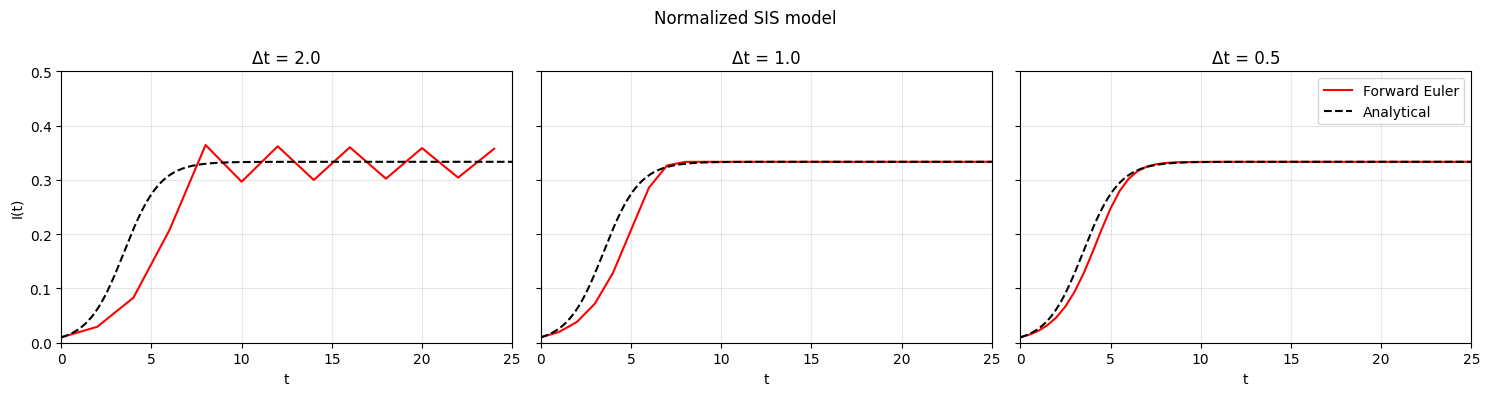
\includegraphics[width=0.8\textwidth]{SIS-simulation.png}
	 \end{center}
	\end{solution}

	\item Comment on what you see in your three plots. How does the step size affect our solution?

	\begin{solution}
		What I notice here is that the smaller the step size, the more accurate the simulation is. 
		The largest step size of 2 showed a curve with much more variance than the analytical solution.
		With each decrease in step size, the curves converge more and more towards each other.
	\end{solution}

	\item Define the maximum absolute error for a simulation using a particular $\Delta t$ as 
	$$E(\Delta t) = \max_{t} \big | I_{\text{Euler}, \Delta t} (t) - I_\text{analytical}(t) \big |\ .$$ 
	Write a function that runs the appropriate simulation, computes the analytical solution, and returns $E$ without plotting. 
	Share a link to your code for this problem.

	\begin{solution}
		\href{https://github.com/JasonHunter95/infectious-diseases/blob/main/HW2/homework_2.ipynb} {My code for problem 1C}
	\end{solution}

	\item Create a plot on log-log axes showing $E(\Delta t)$ vs $\Delta t$ for values 
	$$\Delta t \in \{2,1,\tfrac{1}{2},\tfrac{1}{4},\tfrac{1}{8},\tfrac{1}{16},\tfrac{1}{32}\}$$

	\begin{solution}
		\begin{center}
			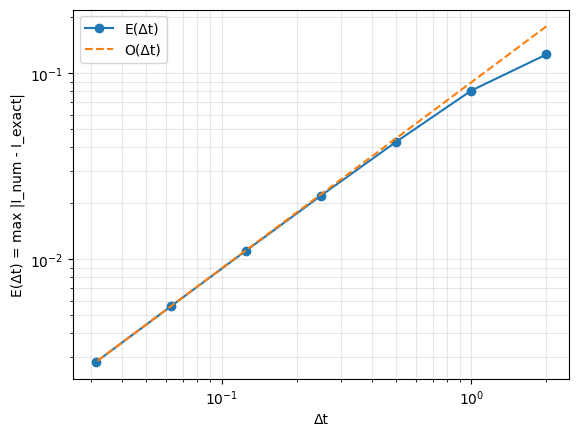
\includegraphics[width=0.8\textwidth]{log-log-error-plot.png}
		\end{center}
	\end{solution}

	\item Comment on what you observe in this plot, and comment on cases when you would want a larger or smaller step size, and why?
	 Imagining yourself in an advisory position in your community, 
	 can you think of any scenario where there is a connection between the step size of your simulation and the ethics of your advice?
		
	\begin{solution}
		The maximum absolute error $E(\Delta t)$ tends to decrease as the step size $\Delta t$ decreases. 
		This further supports what I saw earlier that smaller step sizes lead to more accurate simulations.

	\end{solution}

\end{enumerate}

\clearpage
	\item The goal of this problem is to get you thinking about the constraints on population contact structure and contact matrices, as well as sensitivity analyses.
	
\begin{enumerate}[label=\alph*.]
	\item As one who is interested in modeling disease transmission on college campuses, you hire two teams to measure contact patterns on a nearby campus. The first team, led by Dan Pemic, tells you that there are $200$ faculty and $1800$ students, with a contact matrix of 
	$$C_\text{Pemic} = \begin{pmatrix}
		3.1 & 43.5 \\
		4.7 & 25.0
	\end{pmatrix}$$
The second team, led by Flynn Uenza, tells you that there are $210$ faculty and $1750$ students, with a contact matrix of
	$$C_\text{Uenza} = \begin{pmatrix}
		3.0 & 44.5 \\
		4.8 & 25.1
		\end{pmatrix}
	$$
Whom do you trust more, Dan Pemic or Flynn Uenza? To answer this question, consider the self-consistency (or lack thereof) of each dataset. Explain your reasoning in words and include any calculations used to arrive at your conclusions. 

\item A straightforward fix to self-consistency issues is to ``symmetrize'' the rates. First, we compute the implied total number of intergroup contacts from faculty to students, and then compute the same from students to faculty. After averaging those two counts, divide by the appropriate population size to get per-person rates. Use this approach to symmetrize the two contact matrices. 

\item How different are these two symmetrized matrices, really? Answer the question by computing the ratio of $R_0$ under Pemic's data to $R_0$ under Uenza's data, assuming SIR models with otherwise identical parameters.

\end{enumerate}

\clearpage
\item (Grad / EC): The goal of this problem is to get you to think about additional flavors of models that build on the SIR model backbone, and practice writing down flow diagrams and systems of differential equations. For each of the following situations please (i) draw a flow diagram with the SIR backbone in black, (ii) include any modifications in a second color, and (iii) write out your differential equations using the same color scheme. 
\begin{enumerate}
	\item Suppose that we want to model the possibility that the natural history of infection means that a person is infected {\it but not infectious} before becoming infected-and-infectious. Let the typical {\it latent} period---the time between exposure and infectiousness---last for $q$ days. Use the letter $E$ for this new compartment. Draw a flow diagram for the non-normalized system, and write a set of corresponding differential equations. 
	\item Suppose that we want to model Hospitalization, with the following assumption: Infected folks either recover directly {\it or} they are hospitalized first and then recover. Let the direct recovery rate be $\gamma$, and suppose that there are 4 direct recoveries for every 1 hospitalization. Let the typical duration of a hospitalization be $\delta$ days. Use the letter $h$ for the hospitalized compartment. Draw a flow diagram for the normalized system, and write a set of corresponding differential equations. You should assume that folks in the hospital do not come into contact with anyone else during their hospital stay.
	\item Suppose that we want to model an infectious disease that afflicts a growing population of bacteria, such that the infection follows an SIR model, the bacteria grow according to a logistic growth model with intrinsic growth rate $\alpha$ and carrying capacity $K$. Let all bacteria reproduce, but suppose that susceptible and recovered bacteria produce susceptible progeny, while infected bacteria produce infected progeny. The carrying capacity is shared by all three bacteria. 
\end{enumerate}

\end{enumerate}

\end{document}